\documentclass[aspectratio=169, table]{beamer}

\usepackage[utf8]{inputenc}
\usepackage{listings} 

\usetheme{Pradita}

\subtitle{IF140303-Web Application Development}

\title{Session-02:\\
\vspace{10pt}
\Huge{Pattern Matching}
%\vspace{5pt}
}

\date[Serial]{\\\vspace{15pt}\scriptsize {PRU/SPMI/FR-BM-18/0222}}
\author[Pradita]{\small{\textbf{Alfa Yohannis}}}

\lstdefinelanguage{Elixir} {
	keywords={case, def, defmodule, do, end, for, if, else, true, false},
	basicstyle=\ttfamily\small,
	keywordstyle=\color{blue}\bfseries,
	ndkeywords={@moduledoc, iex, Enum, @doc},
	ndkeywordstyle=\color{purple}\bfseries,
	sensitive=true,
	numbers=left,
	numberstyle=\tiny\color{gray},
	breaklines=true,
	frame=lines,
	backgroundcolor=\color{lightgray!10},
	tabsize=2,
	comment=[l]{\#},
	morecomment=[s]{/*}{*/},
	commentstyle=\color{gray}\ttfamily,
	showstringspaces=false,
	% string settings
	morestring=[b]",
	morestring=[b]',
	stringstyle=\color{black}\ttfamily, % default, will be overridden
	moredelim=[s][\color{blue}\ttfamily]{"}{"},   % double quotes
	moredelim=[s][\color{teal}\ttfamily]{'}{'}    % single quotes
}


\lstdefinelanguage{bash} {
	keywords={},
	basicstyle=\ttfamily\small,
	keywordstyle=\color{blue}\bfseries,
	ndkeywords={iex},
	ndkeywordstyle=\color{purple}\bfseries,
	sensitive=true,
	commentstyle=\color{gray},
	stringstyle=\color{red},
	numbers=left,
	numberstyle=\tiny\color{gray},
	breaklines=true,
	frame=lines,
	backgroundcolor=\color{lightgray!10},
	tabsize=2,
	comment=[l]{\#},
	morecomment=[s]{/*}{*/},
	commentstyle=\color{gray}\ttfamily,
	stringstyle=\color{purple}\ttfamily,
	showstringspaces=false
}

\begin{document}
	
	\frame{\titlepage}
	
		\begin{frame}[fragile]
		\frametitle{Contents}
		\vspace{20pt}
		\begin{columns}[t]
			\column{0.5\textwidth}
			\tableofcontents[sections={1-5}]
			
			\column{0.5\textwidth}
			\tableofcontents[sections={6-20}]
		\end{columns}
	\end{frame}

\section{Relationship between Elixir, Erlang, and BEAM}

\begin{frame}{Relationship between Elixir, Erlang, and BEAM}
\vspace{20pt}
The diagram below shows how Elixir builds on Erlang and both run on BEAM.

\begin{center}
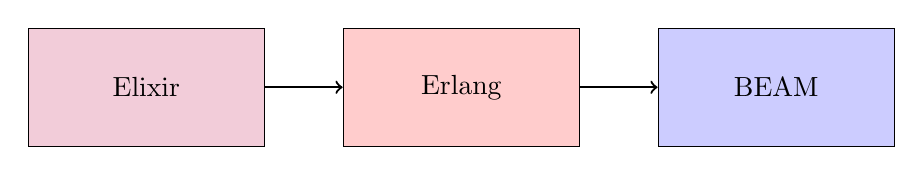
\begin{tikzpicture}[node distance=4cm]
	\node (elixir) [rectangle, draw, text centered, minimum height=1.5cm, minimum width=3cm, fill=purple!20] {Elixir};
	\node (erlang) [rectangle, draw, right of=elixir, text centered, minimum height=1.5cm, minimum width=3cm, fill=red!20] {Erlang};
	\node (beam) [rectangle, draw, right of=erlang, text centered, minimum height=1.5cm, minimum width=3cm, fill=blue!20] {BEAM};
	
	\draw[->, thick] (elixir) -- (erlang);
	\draw[->, thick] (erlang) -- (beam);
\end{tikzpicture}
\end{center}

\textbf{Explanation:}  
When a developer writes Elixir code, it is first translated into Erlang bytecode.  
This bytecode then runs on BEAM, the Erlang Virtual Machine, which efficiently  
manages execution with concurrency, fault tolerance, and distribution.  
Although Elixir and Erlang have different syntax, they share the same runtime,  
making them highly compatible and interoperable.
\end{frame}



\begin{frame}{Elixir, Erlang, and BEAM}
\vspace{20pt}
\begin{columns}[t]
  \column{0.33\textwidth}
  \textbf{Elixir}  
  \begin{itemize}
    \item Modern, dynamic language.  
    \item Built for scalable, fault-tolerant apps.  
    \item Depends on Erlang ecosystem.  
  \end{itemize}

  \column{0.33\textwidth}
  \textbf{Erlang}  
  \begin{itemize}
    \item Foundation language for Elixir.  
    \item Elixir compiles into Erlang bytecode.  
    \item Provides libraries, tools, frameworks.  
  \end{itemize}

  \column{0.33\textwidth}
  \textbf{BEAM}  
  \begin{itemize}
    \item Erlang Virtual Machine.  
    \item Runs Erlang + Elixir bytecode.  
    \item Supports concurrency, distribution, fault tolerance.  
  \end{itemize}
\end{columns}
\end{frame}

\section{Pattern Matching in Elixir}
\begin{frame}{Pattern Matching in Elixir}
\vspace{20pt}
\begin{itemize}
  \item \textbf{Powerful feature.} Pattern matching is one of the most powerful and fundamental aspects of Elixir. It allows developers to match data structures and extract values declaratively.  
  \item \textbf{Different from assignment.} Unlike imperative languages where variables are initialized with values, in Elixir pattern matching is used for comparison and decomposition of data.  
  \item \textbf{Basic operator.} Pattern matching uses the \texttt{=} operator. If both sides match, Elixir binds the right-hand side values to the variables on the left-hand side.  
\end{itemize}
\end{frame}


\begin{frame}[fragile]{Basics of Pattern Matching}
\vspace{17pt}
\begin{columns}[t]

\column{0.5\textwidth}
\textbf{Basic Pattern Matching.}  
Pattern matching uses the \texttt{=} operator to compare the left and right sides of an expression.  
If they match, Elixir binds the value on the right to the variable on the left.

\begin{lstlisting}[language=Elixir]
iex> x = 1
1

iex> 1 = x
1
\end{lstlisting}

The value \texttt{1} is bound to \texttt{x}. Since both sides match, Elixir simply returns \texttt{1}.

\column{0.5\textwidth}
\textbf{Pattern Matching with Tuples.}  
Pattern matching works well with more complex structures like tuples.

\begin{lstlisting}[language=Elixir]
iex> {a, b, c} = {1, 2, 3}
{1, 2, 3}
iex> a
1
iex> b
2
iex> c
3
\end{lstlisting}

The tuple \texttt{\{1, 2, 3\}} matches the pattern \texttt{\{a, b, c\}}, binding each value to the corresponding variable.
\end{columns}
\end{frame}

\begin{frame}[fragile]{Pattern Matching with Lists and Functions}
\vspace{20pt}
\begin{columns}[t]

\column{0.45\textwidth}
\textbf{Pattern Matching with Lists.}  
Pattern matching can be used with lists, splitting them into \texttt{head} (first element) and \texttt{tail} (remaining elements).

\begin{lstlisting}[language=Elixir]
iex> [head | tail] = [1, 2, 3]
[1, 2, 3]
iex> head
1
iex> tail
[2, 3]
\end{lstlisting}

head binds to the first element, while tail  
captures the rest of the list.

\column{0.55\textwidth}
\textbf{Pattern Matching in Functions.}  
Functions can use pattern matching in parameters for clean, declarative code.

\begin{lstlisting}[language=Elixir]
defmodule Example do
  def greet({first, last}) do
    "Hello, #{first} #{last}!"
  end
end

iex> Example.greet({"John", "Doe"})
"Hello, John Doe!"
\end{lstlisting}

greet/1 matches its argument to a tuple,  
automatically binding values to first and last.
\end{columns}
\end{frame}

\begin{frame}[fragile]{Pattern Matching with Conditionals}
\vspace{20pt}
\begin{columns}[t]

\column{0.6\textwidth}
\textbf{Using \texttt{case}.}  
Pattern matching with \texttt{case} enables clean handling of different structures.

\begin{lstlisting}[language=Elixir]
defmodule Example do
  def match_pattern(tuple) do
    case tuple do
      {1, x, 3} -> IO.puts("x is #{x}")
      _ -> IO.puts("No match found")
    end
  end
end

# Function call
Example.match_pattern({1, 2, 3})
\end{lstlisting}

\column{0.4\textwidth}
\textbf{Explanation.}  
\begin{itemize}
  \item If the tuple matches \texttt{\{1, x, 3\}},  
        the value of \texttt{x} is printed.  
  \item If no match occurs, the fallback clause runs.  
\end{itemize}

\textbf{Output:}
\begin{verbatim}
x is 2
\end{verbatim}

Pattern matching makes Elixir code declarative,  
expressive, and easier to reason about.
\end{columns}
\end{frame}

\section{Pipe Operator}

\begin{frame}[fragile]{Pipe Operator in Elixir}
\vspace{20pt}
\textbf{Definition.}  
The \textit{pipe operator} (\texttt{|>}) allows chaining multiple operations  
into a readable flow. It passes the output of one expression  
as the first argument to the next function.

\textbf{Example with Pipes:}
\begin{lstlisting}[language=Elixir]
iex> "hello"
  |> String.upcase()
  |> String.reverse()
"OLLEH"
\end{lstlisting}

\textbf{Equivalent without Pipes:}
\begin{lstlisting}[language=Elixir]
iex> String.reverse(String.upcase("hello"))
"OLLEH"
\end{lstlisting}

This makes code cleaner and avoids deeply nested function calls.
\end{frame}


\begin{frame}[fragile]{Pipe Operator with Lists and Anonymous Functions}
\vspace{20pt}
\begin{columns}[t]

\column{0.5\textwidth}
\textbf{Pipe Operator with Lists.}  
The pipe operator chains list operations in a clear flow.

\begin{lstlisting}[language=Elixir]
iex> [1, 2, 3, 4, 5]
  |> Enum.map(&(&1 * 2))
  |> Enum.filter(&(&1 > 5))
[6, 8, 10]
\end{lstlisting}

The list is first doubled with \texttt{Enum.map/2},  
then filtered with \texttt{Enum.filter/2} to  
keep only values greater than 5.

\column{0.5\textwidth}
\textbf{Anonymous Functions (\&1, \&2, ...).}  
The \texttt{\&} operator creates anonymous functions,  
where \texttt{\&1}, \texttt{\&2}, etc. are argument placeholders.

\begin{lstlisting}[language=Elixir]
iex> add = &(&1 + &2)
#Function<.../2 in :erl_eval.expr/5>

iex> add.(2, 3)
5
\end{lstlisting}

This defines a function that adds its  
two arguments and returns the result.
\end{columns}
\end{frame}

\begin{frame}[fragile]{Pipe Operator with Multi-Parameter Functions}
\vspace{20pt}
The pipe operator passes the left-hand value as the first argument,  
while other parameters are provided normally.

\begin{lstlisting}[language=Elixir]
defmodule Example do
  def multiply_and_add(x, y, z) do
    x * y + z
  end
end

iex> 5
  |> Example.multiply_and_add(2, 3)
13
\end{lstlisting}

Here, \texttt{5} is piped as the first parameter,  
then multiplied by \texttt{2} and added with \texttt{3}.
\end{frame}


\begin{frame}[fragile]{Pipe Operator with Type Conversion}
\vspace{20pt}
\begin{columns}[t]

\column{0.55\textwidth}
\textbf{Code Example.}

\begin{lstlisting}[language=Elixir]
defmodule Converter do
  def string_to_integer(str) do
    String.to_integer(str)
  end

  def add_five(num) do
    num + 5
  end
end

iex> "42"
  |> Converter.string_to_integer()
  |> Converter.add_five()
47
\end{lstlisting}

\column{0.45\textwidth}
\textbf{Explanation.}  
\begin{itemize}
  \item The pipe operator sends the output of one function as the first argument to the next.  
  \item Here, the string \texttt{"42"} is converted into an integer using \texttt{string\_to\_integer/1}.  
  \item The resulting integer is then passed to \texttt{add\_five/1}, producing \texttt{47}.  
  \item This style avoids nested calls and keeps the transformation steps clear.  
\end{itemize}

\end{columns}
\end{frame}

\begin{frame}[fragile]{Using Pipe as the Second Parameter}
\vspace{20pt}
\begin{columns}[t]

\column{0.55\textwidth}
\textbf{Code Example.}

\begin{lstlisting}[language=Elixir]
defmodule Example do
  def hello(greet, name) do
    greet <> name
  end
end

iex> "world"
  |> (&Example.hello("Hello, ", &1)).()
"Hello, world"
\end{lstlisting}

\column{0.45\textwidth}
\textbf{Explanation.}  
\begin{itemize}
  \item The module \texttt{Example} defines \texttt{hello/2},  
        which concatenates two strings: \texttt{greet} and \texttt{name}.  
  \item The string \texttt{"world"} is piped into an anonymous function.  
  \item Inside the anonymous function, \texttt{"Hello, "} is the first argument,  
        while the piped value (\texttt{"world"}) becomes the second argument.  
  \item The result is \texttt{"Hello, world"}.  
\end{itemize}

\end{columns}
\end{frame}

\section{File Operations}
\begin{frame}[fragile]{Saving Data to a File}
\vspace{20pt}
To save data to a file, use the \texttt{File.write/2} function with a filename and the data.  
If the operation is successful, it returns \texttt{:ok}.  
If it fails (e.g., due to missing permissions), it returns \texttt{:error, reason}.

\begin{lstlisting}[language=Elixir]
filename = "data.txt"
data = "Hello, Elixir!"
File.write(filename, data)
\end{lstlisting}

IEx Output:
\begin{lstlisting}[language=Elixir]
:ok
\end{lstlisting}

This example writes the string \texttt{"Hello, Elixir!"} into a file named  
\texttt{data.txt}. If the file does not exist, it will be created automatically.
\end{frame}


\begin{frame}[fragile]{Reading Data from a File}
\vspace{20pt}
\begin{columns}[t]

\column[t]{0.65\textwidth}
\begin{lstlisting}[language=Elixir]
defmodule FileReader do
  def read_file(filename) do
    case File.read(filename) do
      {:ok, content} ->
        IO.puts("File content: #{content}")
      {:error, reason} ->
        IO.puts("Failed to read file: #{reason}")
    end
  end
end
# Call in IEx
iex> FileReader.read_file("data.txt")
File content: Hello, Elixir!
\end{lstlisting}

\column{0.35\textwidth}
\textbf{Explanation:}
\begin{itemize}
  \item \texttt{File.read/1} returns either \texttt{:ok, content} or \texttt{:error, reason}.
  \item Pattern matching with \texttt{case} handles both success and failure cases.
  \item In this example, the content of \texttt{data.txt} is printed to the console.
  \item If the file is missing, the error reason is displayed instead.
\end{itemize}

\end{columns}
\end{frame}



\begin{frame}[fragile]{Adding Dependency \texttt{\{:jason, "~> 1.4"\}}}
\vspace{20pt}
\begin{columns}[t]

\column{0.4\textwidth}
\textbf{Example in \texttt{mix.exs}:}
\begin{lstlisting}[language=Elixir]
defp deps do
  [
    {:jason, "~> 1.4"}
  ]
end
\end{lstlisting}

\textbf{Fetch the dependency:}
\begin{lstlisting}[language=bash]
mix deps.get
\end{lstlisting}

\column{0.6\textwidth}
\textbf{Explanation:}
\begin{itemize}
  \item Open \texttt{mix.exs} in the root of your project.
  \item Add the dependency inside the \texttt{deps/0} function.
  \item Run \texttt{mix deps.get} to download and install it.
  \item \texttt{Jason} is a fast library for encoding/decoding JSON in Elixir.
\end{itemize}

\end{columns}
\end{frame}


\begin{frame}[fragile]{Saving Data in JSON Format}
\vspace{20pt}
\begin{columns}[t]

\column{0.6\textwidth}
\textbf{Module Example (\texttt{lib/json\_file\_handler.ex}):}
\begin{lstlisting}[language=Elixir, basicstyle=\ttfamily\scriptsize]
defmodule Json_File_Handler do
  # Save data to a JSON file
  def save_json(filename, data) do
    File.write(filename, Jason.encode!(data))
  end
end
\end{lstlisting}

\textbf{IEx Usage:}
\begin{lstlisting}[language=Elixir, basicstyle=\ttfamily\scriptsize]
filename = "data.json"
data = %{"greeting" => "Hello, Elixir!", "count" => 42}
Json_File_Handler.save_json(filename, data)
\end{lstlisting}

\column{0.4\textwidth}
\textbf{Explanation:}
\begin{itemize}
  \item \texttt{Jason.encode!/1} converts Elixir data into JSON format.
  \item \texttt{File.write/2} saves the JSON string into the file.
  \item If the file does not exist, it will be created automatically.
\end{itemize}

\end{columns}
\end{frame}


\begin{frame}[fragile]{Loading Data from JSON Format}
\vspace{20pt}
\begin{columns}[t]

\column{0.67\textwidth}
\textbf{Module Example (\texttt{lib/json\_file\_handler.ex}):}
\begin{lstlisting}[language=Elixir, basicstyle=\ttfamily\scriptsize]
defmodule Json_File_Handler do
  # Load data from a JSON file
  def load_json(filename) do
    case File.read(filename) do
      {:ok, content} ->
        case Jason.decode(content) do
          {:ok, decoded_data} ->
            IO.inspect(decoded_data)
          {:error, reason} ->
            IO.puts("Failed to decode JSON: #{reason}")
        end
      {:error, reason} ->
        IO.puts("Failed to read file: #{reason}")
    end
  end
end
\end{lstlisting}

\column{0.34\textwidth}
\textbf{IEx Usage:}
\begin{lstlisting}[language=Elixir, basicstyle=\ttfamily\scriptsize]
Json_File_Handler.load_json("data.json")
\end{lstlisting}
\textbf{Explanation:}
\begin{itemize}
  \item \texttt{File.read/1} reads the contents of the JSON file.
  \item \texttt{Jason.decode/1} parses JSON text into Elixir data.
  \item Handles both success and error cases with \texttt{case}.
\end{itemize}

\end{columns}
\end{frame}


\section{Exercise}
\begin{frame}[fragile]{Exercise 1: Pattern Matching in Elixir}
\vspace{20pt}

\begin{lstlisting}[language=Elixir, basicstyle=\ttfamily\footnotesize]
# Simple Pattern Matching
{x, y, z} = {1, 2, 3}
IO.puts("x = #{x}, y = #{y}, z = #{z}")

# Pattern Matching with List
[head | tail] = [1, 2, 3, 4, 5]
IO.puts("Head: #{head}")
IO.inspect(tail)

# Pattern Matching with Map
%{name: name, age: age} = %{name: "John", age: 30}
IO.puts("Name: #{name}, Age: #{age}")
\end{lstlisting}

\textbf{Explanation:}  
This exercise shows how Elixir destructures different data structures:  
tuples, lists, and maps. Pattern matching assigns values directly to variables,  
making the code concise and expressive.
\end{frame}


\begin{frame}[fragile]{Exercise 2: Pipe Operator in Elixir}
\vspace{20pt}

\begin{lstlisting}[language=Elixir, basicstyle=\ttfamily\footnotesize]
# Example of Using the Pipe Operator
defmodule PipeExample do
  def greet(name), do: "Hello, " <> name
  def exclaim(statement), do: statement <> "!"
  def emphasize(statement), do: String.upcase(statement)
end

"world"
|> PipeExample.greet()
|> PipeExample.exclaim()
|> PipeExample.emphasize()
|> IO.puts()
\end{lstlisting}

\textbf{Explanation:}  
This exercise demonstrates how the pipe operator \texttt{|>}  
passes the output of one function as the first argument to the next.  
The word \texttt{"world"} is transformed step by step into  
\texttt{"HELLO, WORLD!"}.
\end{frame}

\begin{frame}[fragile]{Pipe Operator with Second Parameter}
\vspace{20pt}

\begin{lstlisting}[language=Elixir, basicstyle=\ttfamily\footnotesize]
defmodule Example do
  def wrap_in_brackets(prefix, content), 
    do: prefix <> "[" <> content <> "]"
end

"world"
|> (&Example.wrap_in_brackets(&1, "Hello")).()
|> IO.puts()
\end{lstlisting}

\textbf{Explanation:}  
Here the pipe operator value is passed as the \textit{second parameter}  
by using an anonymous function. The placeholder \texttt{\&1} refers to the  
value coming through the pipe. Similarly, \texttt{\&2}, \texttt{\&3}, etc.  
refer to subsequent parameters in anonymous functions.
\end{frame}

\begin{frame}[fragile]{Exercise 3: Reading a Text File}
\vspace{20pt}
This exercise uses the \texttt{FileReader} module to read the contents  
of a text file. Make sure \texttt{data.txt} exists with some content inside.

\begin{lstlisting}[language=Elixir, basicstyle=\ttfamily\footnotesize]
# File: lib/file_reader.ex
defmodule FileReader do
  def read_file(filename) do
    case File.read(filename) do
      {:ok, content} ->
        IO.puts("File content: #{content}")
      {:error, reason} ->
        IO.puts("Failed to read file: #{reason}")
    end
  end
end
# usage
iex> FileReader.read_file("data.txt")
File content: Hello, Elixir!
\end{lstlisting}
\end{frame}

\begin{frame}[fragile]{Exercise 4: Saving JSON Data}
\vspace{20pt}
\textbf{Module Example (\texttt{lib/json\_file\_handler.ex}):}
\begin{lstlisting}[language=Elixir, basicstyle=\ttfamily\scriptsize]
defmodule JsonFileHandler do
  # Save data to a JSON file
  def save_json(filename, data) do
    File.write(filename, Jason.encode!(data))
  end
end
\end{lstlisting}

\textbf{IEx Usage:}
\begin{lstlisting}[language=Elixir, basicstyle=\ttfamily\scriptsize]
iex> filename = "data.json"
iex> data = %{"greeting" => "Hello, Elixir!", "count" => 42}
iex> JsonFileHandler.save_json(filename, data)
:ok
\end{lstlisting}
\end{frame}


\begin{frame}[fragile]{Exercise 4: Reading JSON Data}
\vspace{20pt}
\begin{lstlisting}[language=Elixir, basicstyle=\ttfamily\scriptsize]
defmodule JsonFileHandler do
  # Load data from a JSON file
  def load_json(filename) do
    case File.read(filename) do
      {:ok, content} ->
        case Jason.decode(content) do
          {:ok, decoded_data} ->
            IO.inspect(decoded_data)
          {:error, reason} ->
            IO.puts("Failed to decode JSON: #{reason}")
        end
      {:error, reason} ->
        IO.puts("Failed to read file: #{reason}")
    end
  end
end

iex> JsonFileHandler.load_json("data.json")
%{"count" => 42, "greeting" => "Hello, Elixir!"}
\end{lstlisting}
\end{frame}


\begin{frame}[fragile]{Exercise 5: Combining All Concepts (Part 1)}
\vspace{20pt}
\begin{lstlisting}[language=Elixir, basicstyle=\ttfamily\footnotesize]
defmodule IntegratedExercise do
  def process_file(filename) do
    # Read JSON file
    filename
    |> File.read()
    |> case do
      {:ok, content} ->
        # Decode JSON and extract values with pattern matching
        case Jason.decode(content) do
          {:ok, %{"greeting" => greeting, "count" => count}} ->
            # Manipulate data using the pipe operator
            new_count = count + 1
            new_data = %{"greeting" => greeting, "count" => new_count}
			
            # Save new data back to JSON file
            File.write(filename, Jason.encode!(new_data))
\end{lstlisting}
\end{frame}


\begin{frame}[fragile]{Exercise 5: Combining All Concepts (Part 2)}
\vspace{20pt}
\begin{lstlisting}[language=Elixir, basicstyle=\ttfamily\footnotesize]
            
          {:error, reason} ->
            IO.puts("Failed to decode JSON: #{reason}")
        end

      {:error, reason} ->
        IO.puts("Failed to read file: #{reason}")
    end
  end
end

# Call the function
filename = "data.json"
IntegratedExercise.process_file(filename)
\end{lstlisting}
\end{frame}



\begin{frame}{Exercise 5: Combining All Concepts (Part 2)}
\vspace{20pt}
\textbf{Instructions:}
\begin{enumerate}
  \item Create a file \texttt{data.json} with the structure:  
  \texttt{\{"greeting": "Hello, Elixir!", "count": 42\}}.
  \item Run \texttt{IntegratedExercise.process\_file("data.json")}.
  \item Observe that the \texttt{count} value increases by 1 each time.
  \item Modify the function to:
  \begin{itemize}
    \item Add new keys/values to the JSON.
    \item Change existing values (e.g., update the greeting).
  \end{itemize}
  \item Ensure the final result is written back to the same JSON file.
\end{enumerate}

\textbf{Concepts Used:}
\begin{itemize}
  \item Pattern Matching, Pipe Operator, Reading and Writing JSON Files
\end{itemize}
\end{frame}

\begin{frame}[fragile]{Extending the Lottery Module (Part 1)}
\vspace{20pt}
\begin{lstlisting}[language=Elixir, basicstyle=\ttfamily\scriptsize]
defmodule Lottery do
  def generate_pool do
    numbers = ["Number 1", "Number 2", "Number 3", "Number 4", "Number 5"]
    pots = ["Pot 1", "Pot 2", "Pot 3", "Pot 4"]
    # Create pool by combining numbers and pots
    for pot <- pots, number <- numbers do
      "#{number} in #{pot}"
    end
  end

  def randomize(pool) do
    Enum.shuffle(pool)
  end

  def contains?(pool, number) do
    Enum.member?(pool, number)
  end

  def distribute(pool, draw_size) do
    Enum.split(pool, draw_size)
  end
\end{lstlisting}
\end{frame}


\begin{frame}[fragile]{Extending the Lottery Module (Part 2)}
\vspace{20pt}
\begin{lstlisting}[language=Elixir, basicstyle=\ttfamily\scriptsize]
  def save_pool(pool, filename) do
    binary = :erlang.term_to_binary(pool)
    File.write(filename, binary)
  end

  def load_pool(filename) do
    case File.read(filename) do
      {:ok, binary} -> :erlang.binary_to_term(binary)
      {:error, _reason} -> "File not found"
    end
  end

  def create_hand(draw_size) do
    Lottery.generate_pool()
    |> Lottery.randomize()
    |> Lottery.distribute(draw_size)
  end
end
\end{lstlisting}
\end{frame}


\begin{frame}{Function Descriptions}
\vspace{20pt}
\begin{itemize}
  \item \textbf{\texttt{save\_pool/2}}: Converts the lottery pool into binary format and saves it to a file. This allows the pool state to be persisted.
  \item \textbf{\texttt{load\_pool/1}}: Reads the binary file and converts it back into a lottery pool. If the file is not found, it returns an error message.
  \item \textbf{\texttt{create\_hand/1}}: Creates a random lottery hand by generating a pool, shuffling it, and splitting it according to the draw size.
\end{itemize}
\end{frame}


\end{document}
